% !TeX encoding = utf8
% 
% % !TeX spellcheck = fr

\begin{Exo}[name={Devoir},title={Système de pendulation},origin={Adapté de Centrale MP 2000},label={exo:CentralePendulation}]


%Adapté d'un sujet de Pierre Breteau (dossier Partage)


\begin{wrapfigure}[21]{r}{0.55\textwidth}
\centering
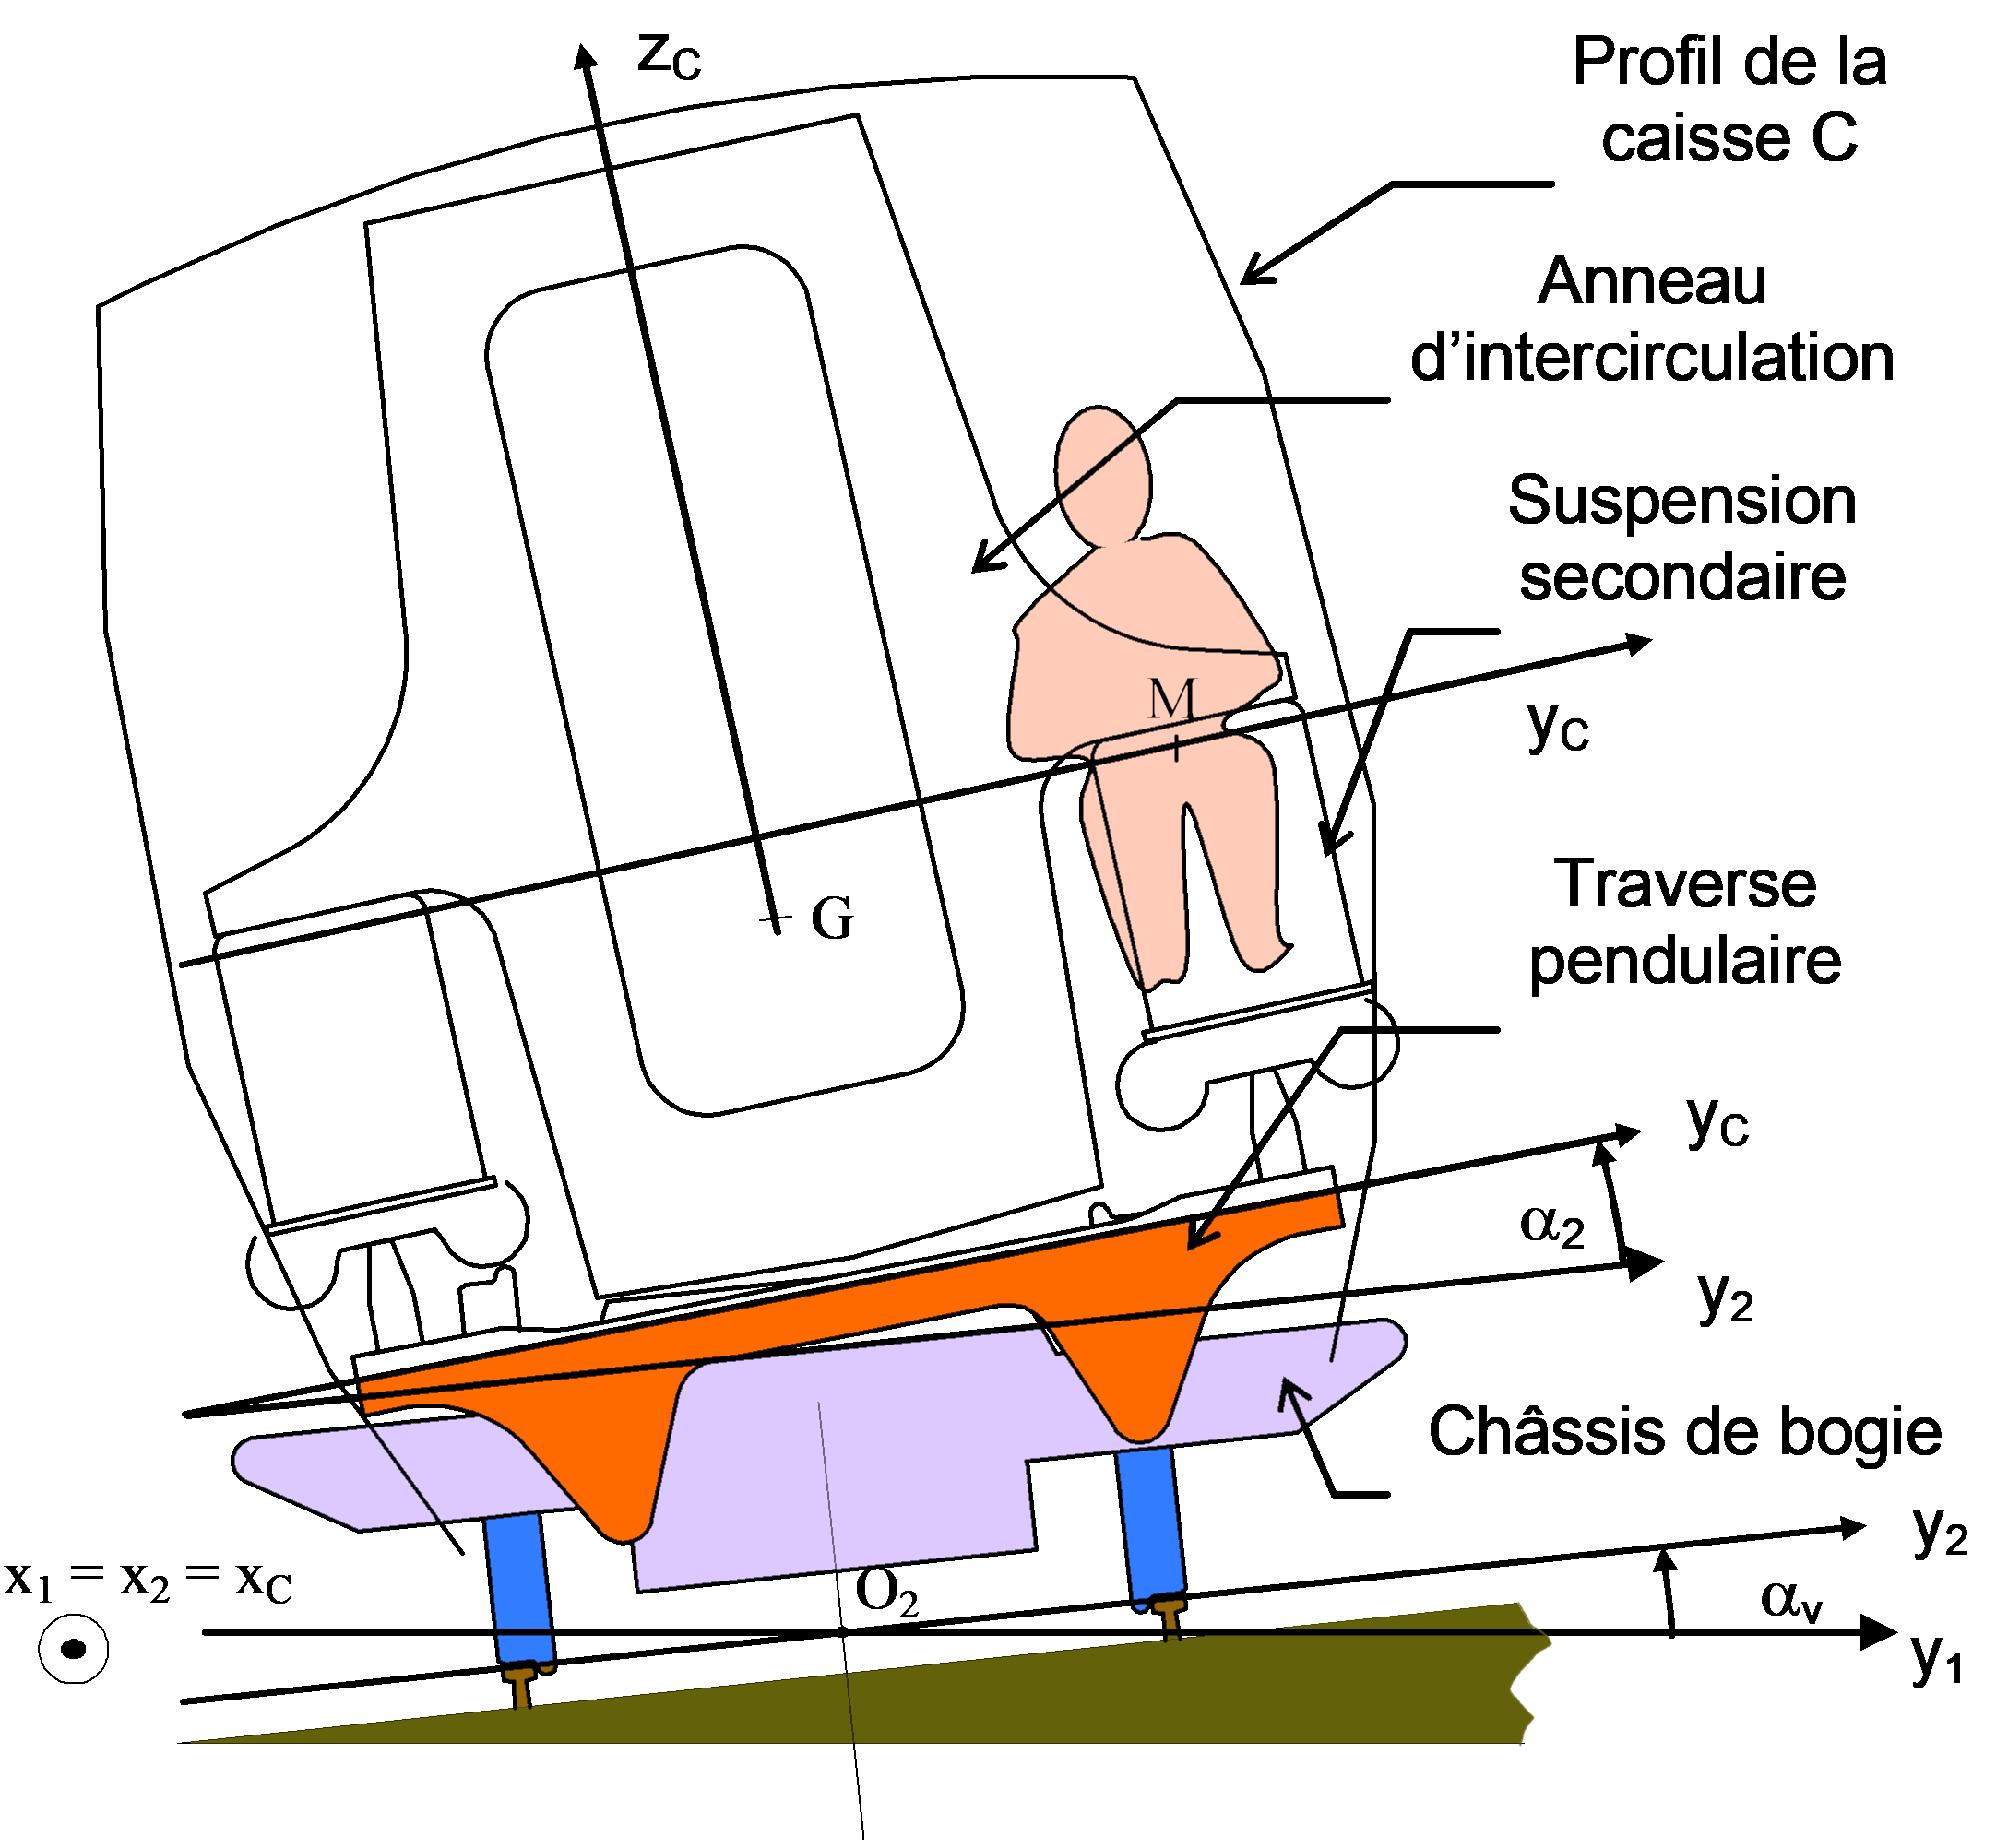
\includegraphics[width=0.55\textwidth]{trainPendulaire-1.png}
\caption{Principe de la pendulation}
\label{fig:trainPenduilaire-1}
\end{wrapfigure}

\partie*{La pendulation}
Afin de compenser les effets centrifuges et d’améliorer le confort des passagers, pour les trains à grande vitesse (TGV), il est nécessaire de contrôler l’inclinaison de la caisse de la voiture par rapport à la voie.

Cette inclinaison résulte de la superposition (figure~\ref{fig:trainPenduilaire-1}) :
\begin{itemize}
\item du devers de voie (inclinaison $\alpha_v$  du bogie par rapport à la voie) 
\item	de la pendulation (inclinaison $\alpha_2$ de la caisse par rapport au bogie) 

\end{itemize}



L’étude proposée concerne un banc d’essais de pendulation (développé par Gec Alstom) qui permet la maîtrise de l’asservissement en inclinaison de la caisse de la voiture par rapport au bogie.

La consigne de position angulaire à obtenir est calculée à partir d’informations provenant de capteurs (accéléromètres\dots) implantés sur les différentes voitures du train. La gestion de ces informations n’est pas abordée dans l’étude proposée. Le modèle retenu correspond à l’étude préliminaire du système qui devra être réalisée sur un banc d’essai fixe.

le système de pendulation active proposée utilise des vérins hydrauliques double effet piloté par une servo-valve pour incliner la caisse.



\begin{wrapfigure}[15]{r}{0.6\textwidth}
\centering
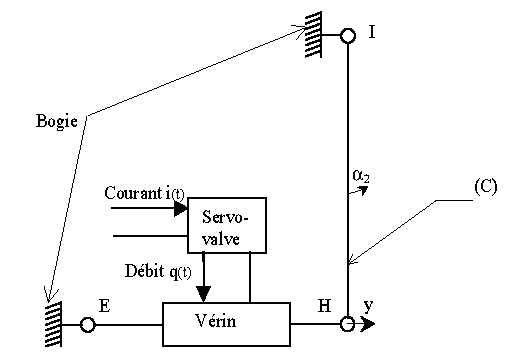
\includegraphics{trainPendulaire-2.pdf}

\caption{Schéma de principe du banc d'essai}
\label{fig:trainPendulaire-2}
\end{wrapfigure}

\partie*{Description du banc d’essais}
La figure~\ref{fig:trainPendulaire-2}   représente le schéma de principe retenu pour l’installation. La charge à déplacer est la caisse de la voiture pendulée qui est modélisée par un solide C mobile en rotation autour de l’axe   par rapport au bogie fixé au banc d’essai. La servo-valve est un organe commandé par un courant d’intensité $i(t)$   qui permet d’obtenir un débit volumique d’huile  $q(t)$  proportionnel au courant d’alimentation. Ce débit volumique  $q(t)$ alimente un vérin double effet qui permet de déplacer la caisse. Le vérin développe une force $f(t)$  et produit un déplacement de la tige $y(t)$  qui permet la mise en rotation de la caisse (C). 

Un capteur de position permet de connaître la position $y(t)$  de la tige du vérin par rapport au corps de vérin. Un correcteur permet d’élaborer une tension de commande $u(t)$  qui, via un convertisseur tension-courant, génère le courant $i(t)$ qui alimente la servo-valve.


Notation des transformées de Laplace

\begin{tabular}{|c|c|c|}\hline
Notation	& 	Désignation					&	Transformée de Laplace \\ \hline
$u_c(t)$	& Tension de consigne	 		&	$U_c(p)$ \\
 
$i(t)$ 		& Courant de commande de la servo-valve	 & $I(p)$ \\
 
$q(t)$ 		& Débit volumique sortant de la servo-valve	 & $Q(p)$ \\
 
$\delta_p(t)=p_A(t)-p_B(t)$
			& Pression utile dans le vérin	 & $\Delta_p(p)$ \\
 
$y(t)$		&Position de la tige du vérin	 	& $Y(p)$ \\
 
$v(t)$		& Vitesse de sortie de la tige du vérin	 & $V(p)$\\
 
$\gamma(t)$	&Accélération de sortie de la tige du vérin	 & $\Gamma(p)$ \\
 
$\alpha_2(t)$ & Position angulaire de la caisse	 		& $A_2(p)$ \\
 
$f(t)$			& Force exercée par le vérin					& $F(p)$\\ \hline
\end{tabular}

Données

 \begin{tabular}{|c|c|c|}\hline
Notation	& 	Désignation					&	Unité \\ \hline
$V_0$	&	Volume initial dans la chambre A du vérin & \si{\metre^3} \\

$R$		& Hauteur de la caisse						& \si{\metre} \\

$J$			&	Moment d'inertie de la caisse par rapport à l'axe & \si{\kilogram\metre\tothe{2}}\\
 
$S$		& Section du piston du vérin					& \si{\metre^2}\\
 
$b$     	& Module de compressibilité de l'huile		& \si{\pascal} \\
 
$\mu$		& Coefficient de couple de rappel	 &  \si{\newton\metre\per\radian} \\ \hline
\end{tabular}
	 
 \partie{Modèle de connaissance}
 
 Le modèle de connaissance est décrit par les équations ci-dessous.
 \begin{itemize}
\item  Le fluide est considéré comme compressible. Le débit $q(t)$  délivré par la servo-valve et entrant dans le vérin est relié à la pression utile $\delta_p(t)$   existant dans le vérin par l'équation :
 \begin{align*}
q(t)&=2\cdot S\cdot v(t)+\dfrac{V_0}{b}\cdot \difft{\delta_p(t)}
\end{align*}
\item L'effort exercé par le vérin sur la caisse est noté  $f(t)$   et vaut :  
\begin{align*}
f(t)&= S\cdot \delta_p(t)
\end{align*}
\item 	L'étude  dynamique de la caisse C permet d'écrire la relation :
\begin{align*}
J\cdot \difftt{\alpha_2(t)}&=f(t)\cdot R-\mu \cdot \alpha_2(t)
\end{align*}
\item Les déplacements sont de faibles amplitudes :  	
\begin{align*}
y(t) =R\cdot \alpha_2(t)
\end{align*}
\item 	La vitesse de déplacement de la tige $v(t)$   est donnée par:
\begin{align*}
v(t)&=\difft{y(t)}
\end{align*}

\end{itemize}


\clearpage


\qst Écrire les 5 équations du modèle de connaissance dans le domaine de Laplace.


\Acompleter[15]


\qst Compléter le schéma-blocs



\begin{tikzpicture}
\sbEntree{Q}
\sbComp{C1}{Q}				\sbRelier[$Q(p)$]{Q}{C1}
\sbBlocL{B1}{- - - - - - - - - -  }{C1}
\sbBloc[3]{B2}{- - - - - - - - - - }{B1}			\sbRelier[$\Delta_p(p)$]{B1}{B2}
\sbBloc[3]{B3}{- - - - - - - - - - }{B2}
									\sbRelier[$F(p)$]{B2}{B3}
\sbBloc{B4}{- - - - - - - - - - }{B3}
									\sbRelier[$V(p)$]{B3}{B4}
\sbSortie{Y}{B4}					\sbRelier[$Y(p)$]{B4}{Y}

\sbDecaleNoeudy[4]{B3}{R1}
\sbBlocr{R1}{- - - - - - - - - - }{R1}
									\sbRelieryx{B3-B4}{R1}
									\sbRelierxy{R1}{C1}

\end{tikzpicture}


Pour la suite, on considère que le schéma-blocs est:

{\centering

\begin{tikzpicture}
\sbEntree{Q}
\sbComp{C1}{Q}				\sbRelier[$Q(p)$]{Q}{C1}
\sbBlocL{B1}{$\dfrac{b\cdot R^2}{p\cdot V_0\cdot(\mu+J\cdot p^2)}$}{C1}

\sbSortie[5]{Y}{B1}					\sbRelier[$Y(p)$]{B1}{Y}

\sbDecaleNoeudy[4]{B1}{R1}
\sbBlocr[0]{R1}{$2\cdot S\cdot p$}{R1}
									\sbRelieryx{B1-Y}{R1}
									\sbRelierxy{R1}{C1}

\end{tikzpicture}\par

}



\qst Déterminer la fonction de transfert $H_y(p)=\dfrac{Y(p)}{Q(p)}$.

\Acompleter[8]


\qst Mettre $H_y(p)$  sous la forme $H_y(p)=\dfrac{K_y}{p\cdot \left(1+\dfrac{p^2}{\omega_1^2}\right)}$. Déterminer $K_y$  et $\omega_1$, préciser les unités.

\Acompleter[8]


On applique à l'entrée, un échelon de pression $q(t)=Q_0\cdot \heav$.

\qst Déterminer $Q(p)$  puis $Y(p)$.

\Acompleter[8]


\qst Montrer que $Y(p)$  s'écrit $Y(p)=\dfrac{A}{ \left(1+\dfrac{p^2}{\omega_1^2}\right)} +\dfrac{B}{p^2}$

\Acompleter[8]



\qst À partir du tableau des transformées de Laplace:
\sq Déterminer $y(t)$.  
\sq Tracer l'allure de $y(t)$.
\sq Que peut-on dire de $\lim\limits_{y\to\infty}(y(t))$?

\Acompleter[12]



\partie*{Asservissement de position}

On constate qu'il est nécessaire de stabiliser le système afin de le rendre fonctionnel, on propose donc un asservissement qui comporte une boucle de vitesse et une boucle de position (figure~\ref{fig:trainPendulaire-3}).

Les deux boucles sont corrigées par deux correcteurs proportionnels, un pour la boucle interne de vitesse $C_2(p)=K_v$  et l'autre sur le boucle de position $C_1(p)=K_p$.  Un filtre dérivateur est placé sur la boucle de retour $(1+\tau\cdot p)$.


\begin{figure}[!htb]
\centering
{\smaller
\begin{tikzpicture}
\sbEntree{Yc}
\sbBloc[3]{Ad}{$A_d$}{Yc}		\sbRelier[$Y_c(p)$]{Yc}{Ad}
\sbComp[2]{C1}{Ad}				\sbRelier{Ad}{C1}
\sbBlocL{Cor1}{$C_1(p)=K_p$}{C1}
\sbComp{C2}{Cor1}				\sbRelier[$U_v(p)$]{Cor1}{C2}
\sbBlocL{Cor2}{$C_2(p)=K_v$}{C2}	\sbRelier{C2}{Cor2}
\sbBloc{A}{$A$}{Cor2}			\sbRelier[$U(p)$]{Cor2}{A}
\sbBloc{G}{$G$}{A}				\sbRelier[$I(p)$]{A}{G}
\sbBloc{H1}{$\dfrac{\delta}{1+\dfrac{p^2}{\beta^2}}$}{G}
									\sbRelier[$Q(p)$]{G}{H1}
\sbBloc{int}{$\dfrac{1}{p}$}{H1}
									\sbRelier[$V(p)$]{H1}{int}
\sbSortie{Y}{int}					\sbRelier[$Y(p)$]{int}{Y}

\sbDecaleNoeudy[4]{H1}{R1}
\sbBlocr{R1}{$g$}{R1}			\sbRelieryx{H1-int}{R1}
\sbBlocr{R2}{$1+\tau\cdot p$}{R1}
									\sbRelier{R1}{R2}
									\sbRelierxy{R2}{C2}
\sbDecaleNoeudy[4]{R1}{R3}
\sbBlocr{R3}{$h$}{R3}			\sbRelieryx{int-Y}{R3}
									\sbRelierxy{R3}{C1}
\end{tikzpicture}\par
}

 $h=\SI{50}{\volt\per\metre}$, $\delta=\SI{28.1}{\metre\tothe{-2}}$, $\beta=\SI{77}{\radian\per\second}$, $g=\SI{10}{\volt\per\metre\per\second}$, $A\cdot G=\dfrac{1}{300}\si{\metre\tothe{3}\per\second\per\volt}$.
\caption{Asservissement de vitesse et position}
\label{fig:trainPendulaire-3}
\end{figure}

\subpartie*{Boucle de vitesse}

On s’intéresse à la correction de la boucle de vitesse  entre $U_v(p)$ (consigne de  vitesse  en \si{\volt})  et $V(p)$(vitesse en \si{\metre\per\second}). Le schéma figure~\ref{fig:trainPendulaire-3} 
montre que cette correction est réalisée par l’ensemble constitué d’un correcteur
proportionnel $C_2(p)=K_v$  et d’un terme $1+\tau\cdot p$   placé  en aval du capteur de vitesse.


\qst Reproduire le schéma-blocs limité à cette boucle. Préciser la chaîne directe et la chaîne de retour.



\Acompleter[12]



\qst Déterminer la fonction de transfert : $H_v(p)=\dfrac{V(p)}{U_v(p)}$



\Acompleter[12]

Compte tenu des valeurs numériques et quelques arrondis, on obtient:

\begin{align*}
H_v(p)&=\dfrac{\num{0.094}\cdot K_v}{1+\num{0.94}\cdot K_v}\dfrac{1}{1+\dfrac{\num{0.94}\cdot K_v\cdot\tau}{1+\num{0.94}\cdot K_v}\cdot p+\dfrac{p^2}{(1+\num{0.94}\cdot K_v)\cdot\beta^2}}
\end{align*}


Le comportement de la boucle de vitesse va dépendre du couple $(K_v,\tau)$.  On retrouve sur la figure~\ref{fig:trainPendulaire-reptemp}  la réponse temporelle de $v(t)$  pour une consigne de $u_v(t)=U_0\cdot \heav$ avec $U_0=\SI{10}{\volt}$  et différentes valeurs pour le couple $(K_v,\tau)$.

\qst Déterminer pour chaque réponse temporelle, $T_{5\%}$: le temps de réponse à 5\%, $D_{1\%}$: le premier dépassement relatif  et la valeur finale.

\Acompleter[6]



\clearpage



\begin{figure}[H]
\centering

\subfloat[$\tau =\SI{0.42e-2}{\second}$, $K_v = 42$]{

\begin{tikzpicture}[xscale=180,yscale=7]

\draw[xstep=0.005,ystep=0.05,green] (0,0) grid (0.04,1.2);

\draw[-latex] (0,0) -- (0.042,0)node[above](t){$t$};
\draw[-latex] (0,0) -- (0,1.25)node[ right]{$v(t)$};
%\draw[dashed,blue,ultra thick] (0,1) -- (0.05,1);

\RepTemp[color=black,samples=100,smooth,ultra thick,name path=S
]{0:0.04}{
10*(0.975e-1-0.974e-1*exp(-492.*x)*cosh(40.3*x)-1.19*exp(-492.*x)*sinh(40.3*x))
}

\foreach \nn in {0,1,...,4}{
\node[below]at (0.0\nn,0){\num{0.0\nn}};
}
\foreach \nn in {0.2, 0.4, 0.6, 0.8,1,1.2}{
\node[left]at (0,\nn){\num{\nn}};
}

%\draw[dashed,red, name path=D95,ultra thick] (0,0.95) node[left]{$\num{0.95}$}--++ (0.05,0);
%\draw[dashed,red, name path=D105,ultra thick] (0,1.05) node[left]{$\num{1.05}$}--++ (0.05,0);
%

%\path [name intersections={of=D95 and S,by=E}];
%\path [name intersections={of=D105 and S}];
%\draw (E) -- (E|-0,0) node[below=1em]{$T_{5\%}\approx\SI{0.01}{\second}$};

\node[fill=white, above left=1em and 2em of t,minimum width=2.5cm, minimum height=3cm,text width=4cm]{Valeur finale:  \\[2em]
$T_{5\%}$: \\[2em]
$D_{1\%}$:
};
\end{tikzpicture}
}
\subfloat[$\tau =\SI{0.42e-2}{\second}$, $K_v = 21$]{

\begin{tikzpicture}[xscale=180,yscale=7]

\draw[xstep=0.005,ystep=0.05,green] (0,0) grid (0.04,1.2);

\draw[-latex] (0,0) -- (0.042,0)node[above](t){$t$};
\draw[-latex] (0,0) -- (0,1.25)node[ right]{$v(t)$};
%\draw[dashed,blue,ultra thick] (0,1) -- (0.05,1);

\RepTemp[color=black,samples=100,smooth,ultra thick,name path=S
]{0:0.04}{
10*(0.952e-1-0.954e-1*exp(-246.*x)*cos(250.*x)-0.938e-1*exp(-246.*x)*sin(250.*x))
}


\foreach \nn in {0,1,...,4}{
\node[below]at (0.0\nn,0){\num{0.0\nn}};
}
\foreach \nn in {0.2, 0.4, 0.6, 0.8,1,1.2}{
\node[left]at (0,\nn){\num{\nn}};
}

%\draw[dashed,red, name path=D95,ultra thick] (0,0.95) node[left]{$\num{0.95}$}--++ (0.05,0);
%\draw[dashed,red, name path=D105,ultra thick] (0,1.05) node[left]{$\num{1.05}$}--++ (0.05,0);
%

%\path [name intersections={of=D95 and S,by=E}];
%\path [name intersections={of=D105 and S}];
%\draw (E) -- (E|-0,0) node[below=1em]{$T_{5\%}\approx\SI{0.01}{\second}$};

\node[fill=white, above left=1em and 2em of t,minimum width=2.5cm, minimum height=3cm,text width=4cm]{Valeur finale:  \\[2em]
$T_{5\%}$: \\[2em]
$D_{1\%}$:
};
\end{tikzpicture}
}


\subfloat[$\tau =\SI{0.21e-2}{\second}$, $K_v = 21$]{

\begin{tikzpicture}[xscale=180,yscale=7]

\draw[xstep=0.005,ystep=0.05,green] (0,0) grid (0.04,1.2);

\draw[-latex] (0,0) -- (0.042,0)node[above](t){$t$};
\draw[-latex] (0,0) -- (0,1.25)node[ right]{$v(t)$};
%\draw[dashed,blue,ultra thick] (0,1) -- (0.05,1);

\RepTemp[color=black,samples=100,smooth,ultra thick,name path=S
]{0:0.04}{
10*(0.952e-1-0.952e-1*exp(-123.*x)*cos(328.*x)-0.356e-1*exp(-123.*x)*sin(328.*x))
}


\foreach \nn in {0,1,...,4}{
\node[below]at (0.0\nn,0){\num{0.0\nn}};
}
\foreach \nn in {0.2, 0.4, 0.6, 0.8,1,1.2}{
\node[left]at (0,\nn){\num{\nn}};
}

%\draw[dashed,red, name path=D95,ultra thick] (0,0.95) node[left]{$\num{0.95}$}--++ (0.05,0);
%\draw[dashed,red, name path=D105,ultra thick] (0,1.05) node[left]{$\num{1.05}$}--++ (0.05,0);
%

%\path [name intersections={of=D95 and S,by=E}];
%\path [name intersections={of=D105 and S}];
%\draw (E) -- (E|-0,0) node[below=1em]{$T_{5\%}\approx\SI{0.01}{\second}$};

\node[fill=white, above left=1em and 2em of t,minimum width=2.5cm, minimum height=3cm,text width=4cm]{Valeur finale:  \\[2em]
$T_{5\%}$: \\[2em]
$D_{1\%}$:
};
\end{tikzpicture}
}
\subfloat[$\tau =\SI{0.84e-2}{\second}$, $K_v = 42$]{

\begin{tikzpicture}[xscale=180,yscale=7]

\draw[xstep=0.004,ystep=0.05,green] (0,0) grid (0.04,1.2);

\draw[-latex] (0,0) -- (0.042,0)node[above](t){$t$};
\draw[-latex] (0,0) -- (0,1.25)node[ right]{$v(t)$};
%\draw[dashed,blue,ultra thick] (0,1) -- (0.05,1);

\RepTemp[color=black,samples=100,smooth,ultra thick,name path=S
]{0:0.04}{
10*(0.975e-1-0.975e-1*exp(-983.*x)*cosh(852.*x)-.112*exp(-983.*x)*sinh(852.*x))
}


\foreach \nn in {0,1,...,4}{
\node[below]at (0.0\nn,0){\num{0.0\nn}};
}
\foreach \nn in {0.2, 0.4, 0.6, 0.8,1,1.2}{
\node[left]at (0,\nn){\num{\nn}};
}

%\draw[dashed,red, name path=D95,ultra thick] (0,0.95) node[left]{$\num{0.95}$}--++ (0.05,0);
%\draw[dashed,red, name path=D105,ultra thick] (0,1.05) node[left]{$\num{1.05}$}--++ (0.05,0);
%

%\path [name intersections={of=D95 and S,by=E}];
%\path [name intersections={of=D105 and S}];
%\draw (E) -- (E|-0,0) node[below=1em]{$T_{5\%}\approx\SI{0.01}{\second}$};

\node[fill=white, above left=1em and 2em of t,minimum width=2.5cm, minimum height=3cm,text width=4cm]{Valeur finale:  \\[2em]
$T_{5\%}$: \\[2em]
$D_{1\%}$:
};
\end{tikzpicture}
}
\caption{Réponse temporelle de la boucle de vitesse pour une consigne de $u_v(t)=\SI{10}{\volt}$  pour différentes valeurs de $K_v$  et $\tau$.}
\label{fig:trainPendulaire-reptemp}
\end{figure}

On souhaite que cette boucle de vitesse soit la plus rapide possible et que le premier dépassement soit inférieur à 10\%.

\qst Proposer un réglage de $\tau$   et $K_v$.

\Acompleter[8]


Finalement, compte tenu du couple de valeurs choisis, la fonction de transfert $H_v(p)$ devient:
\begin{align*}
H_v(p)&=\dfrac{23250}{(p+488)^2}
\end{align*}

Le schéma-blocs de l'asservissement est représenté sur la figure~\ref{fig:trainPendulaire-4}.






\begin{figure}[H]
\centering
{
\begin{tikzpicture}
\sbEntree{Yc}
\sbBloc[3]{Ad}{$A_d$}{Yc}		\sbRelier[$Y_c(p)$]{Yc}{Ad}
\sbComp[3]{C1}{Ad}				\sbRelier{Ad}{C1}
\sbBloc{Cor1}{$C_1(p)=K_p$}{C1}\sbRelier[$\varepsilon_y(p)$]{C1}{Cor1}
\sbBloc[3]{Hv}{$H_v(p)$}{Cor1}	\sbRelier[$U_v(p)$]{Cor1}{Hv}
\sbBloc[3]{int}{$\dfrac{1}{p}$}{Hv}
									\sbRelier[$V(p)$]{Hv}{int}
\sbSortie{Y}{int}					\sbRelier[$Y(p)$]{int}{Y}

\sbDecaleNoeudy[4]{Hv}{R3}
\sbBlocr{R3}{$h$}{R3}			\sbRelieryx{int-Y}{R3}
									\sbRelierxy{R3}{C1}
\end{tikzpicture}\par
}


\caption{Asservissement de  position}
\label{fig:trainPendulaire-4}
\end{figure}

\qst Quelle doit être la valeur du gain d'adaptation de la consigne $A_d$  pour que l'asservissement fonctionne correctement?

\Acompleter[6]


\qst Modifier le schéma-blocs pour le mettre sous la forme suivante:

{\centering
\begin{tikzpicture}
\sbEntree{Yc}
\sbComp[3]{C1}{Yc}				\sbRelier[$Y_c(p)$]{Yc}{C1}
\sbBloc{BO}{$BO(p)$}{C1}\sbRelier{C1}{BO}
\sbSortie{Y}{BO}					\sbRelier[$Y(p)$]{BO}{Y}

\sbRenvoi[3]{BO-Y}{C1}{}

\end{tikzpicture}\par
}


\qst Déterminer $BO(p)$

\Acompleter[6]


\qst Déterminer la fonction de transfert en boucle fermée $H_p(p)=\dfrac{Y(p)}{Y_c(p)}$  en fonction de $K_p$  et des valeurs numériques.

\Acompleter[10]




Afin d'éviter des oscillations qui pourraient être désagréable pour les passagers  le réglage du correcteur de position est $K_p=\num{0.9}$.

La fonction de transfert devient (avec quelques arrondis!):

\begin{align*}
H_p(p)&=\dfrac{1}{\left(\dfrac{p}{532}+1\right)\cdot \left(\dfrac{p}{439}+1\right)\cdot\left (\dfrac{p}{4.5}+1\right)}
\end{align*}

On sollicite avec un échelon unitaire $y(t)=Y_0\cdot \heav$  avec $Y_0=\SI{0.1}{\metre}$.

\qst Montrer que $Y(p)$  s'écrit 

\begin{align*}
Y(p)= \dfrac{A}{\dfrac{p}{532}+1}+\dfrac{B}{\dfrac{p}{439}+1}+ \dfrac{C}{\dfrac{p}{4.5}+1} +\dfrac{D}{p}
\end{align*}

\Acompleter[12]


\qst Déterminer $y(t)$.

\Acompleter[12]


\qst À partir de la réponse temporelle ci-dessous, préciser, l'erreur indicielle, le temps de réponse.

{\centering
\begin{tikzpicture}[xscale=5,yscale=70]

\draw[xstep=0.2,ystep=0.005,green] (0,0) grid (2,0.12);

\draw[-latex] (0,0) -- (2,0)node[above](t){$t$};
\draw[-latex] (0,0) -- (0,0.125)node[ right]{$y(t)$};
%\draw[dashed,blue,ultra thick] (0,1) -- (0.05,1);

\RepTemp[color=black,samples=100,smooth,ultra thick,name path=S
]{0:2}{
0.1*(1.-0.400e-1*exp(-532.*x)+0.588e-1*exp(-439.*x)-1.02*exp(-4.48*x))
}


\foreach \nn in {0,1,2}{
\node[below]at (\nn,0){\num{\nn}};
}
\foreach \nn in {0.02, 0.04, 0.06, 0.08,0.1,0.12}{
\node[left]at (0,\nn){\num{\nn}};
}

%\draw[dashed,red, name path=D95,ultra thick] (0,0.95) node[left]{$\num{0.95}$}--++ (0.05,0);
%\draw[dashed,red, name path=D105,ultra thick] (0,1.05) node[left]{$\num{1.05}$}--++ (0.05,0);
%

%\path [name intersections={of=D95 and S,by=E}];
%\path [name intersections={of=D105 and S}];
%\draw (E) -- (E|-0,0) node[below=1em]{$T_{5\%}\approx\SI{0.01}{\second}$};

\node[fill=white, above left=1em and 2em of t,minimum width=2.5cm, minimum height=3cm,text width=4cm]{Erreur indicielle:  \\[2em]
$T_{5\%}$: \\[2em]
$D_{1\%}$:
};
\end{tikzpicture}
\par}


\qst Montrer que la fonction de transfert en boucle fermée obtenue peut être simplifiée par \begin{align*}
H_{ps}(p) &=\dfrac{1}{\dfrac{p}{4.5}+1}
\end{align*}

\Acompleter[82]


%
%\begin{align*}
%H_v(p)=\dfrac{550.\cdot Kv}{p^2+5500\cdot K_v\cdot \tau\cdot p+5900+5500\cdot K_v}
%\end{align*}

\begin{Cor}

\begin{multicols}{2}


\qst Écrire les 5 équations du modèle de connaissance dans le domaine de Laplace.

 \begin{align*}
Q(p)&=2\cdot S\cdot V(p)+\dfrac{V_0}{b}\cdot p\cdot \Delta(p)
\end{align*}


\begin{align*}
F(p)&= S\cdot \Delta_p(p)
\end{align*}

\begin{align*}
J\cdot p^2 \cdot A_2(p) &=F(p)\cdot R-\mu \cdot A_2(p)
\end{align*}
soit
\begin{align*}
\left(J\cdot p^2 +\mu \right)\cdot A_2(p)&=F(p)\cdot R
\end{align*}


\begin{align*}
Y(p)=R\cdot A_2(p)
\end{align*}

\begin{align*}
V(p)&=p\cdot Y(p)
\end{align*}

\qst Compléter le schéma-blocs



\begin{tikzpicture}
\sbEntree{Q}
\sbComp[2]{C1}{Q}				\sbRelier[$Q(p)$]{Q}{C1}
\sbBlocL[2]{B1}{$\dfrac{b}{p\cdot V_0}$}{C1}
\sbBloc[2]{B2}{$S$}{B1}			\sbRelier[$\Delta_p(p)$]{B1}{B2}
\sbBloc[2]{B3}{$\dfrac{p\cdot R^2}{\mu+J\cdot p^2}$}{B2}
									\sbRelier[$F(p)$]{B2}{B3}
\sbBloc{B4}{$\dfrac{1}{p}$}{B3}
									\sbRelier[$V(p)$]{B3}{B4}
\sbSortie{Y}{B4}					\sbRelier[$Y(p)$]{B4}{Y}

\sbDecaleNoeudy[4]{B3}{R1}
\sbBlocr{R1}{$2\cdot S$}{R1}
									\sbRelieryx{B3-B4}{R1}
									\sbRelierxy{R1}{C1}

\end{tikzpicture}


Pour la suite, on considère que le schéma-blocs est:

\begin{tikzpicture}
\sbEntree{Q}
\sbComp[1]{C1}{Q}				\sbRelier[$Q(p)$]{Q}{C1}
\sbBlocL[1.5]{B1}{$\dfrac{b\cdot R^2}{p\cdot V_0\cdot(\mu+J\cdot p^2)}$}{C1}

\sbSortie[5]{Y}{B1}					\sbRelier[$Y(p)$]{B1}{Y}

\sbDecaleNoeudy[4]{B1}{R1}
\sbBlocr[0]{R1}{$2\cdot S\cdot p$}{R1}
									\sbRelieryx{B1-Y}{R1}
									\sbRelierxy{R1}{C1}

\end{tikzpicture}


\qst Déterminer la fonction de transfert $H_y(p)=\dfrac{Y(p)}{Q(p)}$.

\begin{align*}
H_y(p)&=\dfrac{Y(p)}{Q(p)}=\dfrac{CD(p)}{1+CD(p)\cdot CR(p)}\\
H_y(p)&=\dfrac{\dfrac{b\cdot R^2}{p\cdot V_0\cdot(\mu+J\cdot p^2)}}
{1+\dfrac{b\cdot R^2\cdot2\cdot S\cdot p}{p\cdot V_0\cdot(\mu+J\cdot p^2)}}\\
H_y(p)&=\dfrac{b\cdot R^2}
{{p\cdot V_0\cdot(\mu+J\cdot p^2)}+2\cdot b\cdot R^2\cdot S\cdot p}\\
H_y(p)&=\dfrac{b\cdot R^2}
{p\cdot \left( V_0\cdot\mu+2\cdot b\cdot R^2\cdot S+V_0\cdot J\cdot p^2\right)}\\
H_y(p)&=\dfrac{\dfrac{b\cdot R^2}{V_0\cdot\mu+2\cdot b\cdot R^2\cdot S}}
{p\cdot \left( 1+\dfrac{V_0\cdot J}{V_0\cdot\mu+2\cdot b\cdot R^2\cdot S}\cdot p^2\right)}
\end{align*}



\qst Mettre $H_y(p)$  sous la forme $H_y(p)=\dfrac{K_y}{p\cdot \left(1+\dfrac{p^2}{\omega_1^2}\right)}$. Déterminer $K_y$  et $\omega_1$, préciser les unités.

\begin{align*}
H_y(p)&=\dfrac{\dfrac{b\cdot R^2}{V_0\cdot\mu+2\cdot b\cdot R^2\cdot S}}
{p\cdot \left( 1+\dfrac{V_0\cdot J}{V_0\cdot\mu+2\cdot b\cdot R^2\cdot S}\cdot p^2\right)}
\end{align*}

On pose
\begin{align*}
K_y&=\dfrac{b\cdot R^2}{V_0\cdot\mu+2\cdot b\cdot R^2\cdot S}\\
\omega_1&=\sqrt{ \dfrac{V_0\cdot\mu+2\cdot b\cdot R^2\cdot S}{V_0\cdot J} }
\end{align*}
avec 
$K_y$  en \si{\metre\tothe{-2}\second}.
et 
$\omega_1$  en $\si{\second\tothe{-1}}$.



On applique à l'entrée, un échelon de pression $q(t)=Q_0\cdot \heav$.

\qst Déterminer $Q(p)$  puis $Y(p)$.

\begin{align*}
Q(p)&=\dfrac{Q_0}{p}
\end{align*}

d'où

\begin{align*}
Y(p)&=\dfrac{K_y}{p\cdot \left(1+\dfrac{p^2}{\omega_1^2}\right)}\cdot \dfrac{Q_0}{p}
\end{align*}


\qst Montrer que $Y(p)$  s'écrit $Y(p)=\dfrac{A}{ \left(1+\dfrac{p^2}{\omega_1^2}\right)} +\dfrac{B}{p^2}$


\begin{align*}
%Y(p)&=\dfrac{K_y}{p\cdot \left(1+\dfrac{p^2}{\omega_1^2}\right)}\cdot \dfrac{Q_0}{p}\\
Y(p)&=\dfrac{A}{ \left(1+\dfrac{p^2}{\omega_1^2}\right)} +\dfrac{B}{p^2}=\dfrac{A\cdot p^2+B\cdot\left(1+\dfrac{p^2}{\omega_1^2}\right)}{p^2\cdot \left(1+\dfrac{p^2}{\omega_1^2}\right)}\\
Y(p)&==\dfrac{A\cdot p^2+B+\dfrac{B}{\omega_1^2}\cdot p^2}{p^2\cdot \left(1+\dfrac{p^2}{\omega_1^2}\right)}=\dfrac{K_y}{p\cdot \left(1+\dfrac{p^2}{\omega_1^2}\right)}\cdot \dfrac{Q_0}{p}
\end{align*}

On déduit:
\begin{align*}
B&=K_y\cdot Q_0\\
A&=-\dfrac{B}{\omega_1^2}=-\dfrac{K_y\cdot Q_0}{\omega_1^2}
\end{align*}


\qst À partir du tableau des transformées de Laplace:
\sq Déterminer $y(t)$.  

On lit sur le tableau:
\begin{align*}
\dfrac{B}{p^2} &\xrightarrow{\mathrm{L}^{-1}} B\cdot t\cdot \heav
\end{align*}
et
\begin{align*}
\dfrac{\omega}{p^2 -\omega^2} &\xrightarrow{\mathrm{L}^{-1}} \sin\left(\omega\cdot t\right)\cdot \heav
\end{align*}
\begin{align*}
\dfrac{A}{ \left(1+\dfrac{p^2}{\omega_1^2}\right)}& = -\dfrac{K_y\cdot Q_0}{\omega_1^2}\cdot \dfrac{1}{ \left(1+\dfrac{p^2}{\omega_1^2}\right)}\\
\dfrac{A}{ \left(1+\dfrac{p^2}{\omega_1^2}\right)}& = - \dfrac{K_y\cdot Q_0}{ \left(\omega_1^2+{p^2}\right)}
\end{align*}
d'où
\begin{align*}
\dfrac{A}{ \left(1+\dfrac{p^2}{\omega_1^2}\right)}&\xrightarrow{\mathrm{L}^{-1}} \dfrac{K_y\cdot Q_0}{\omega_1}\cdot \sin\left(\omega_1\cdot t\right)\cdot \heav
\end{align*}
finalement
\begin{align*}
y(t)&=\left(B\cdot t-\dfrac{K_y\cdot Q_0}{\omega_1}\cdot \sin\left(\omega_1\cdot t\right)\right)\heav
\end{align*}


\sq Tracer l'allure de $y(t)$.

La réponse temporelle est la superposition d'un sinus et d'une rampe.

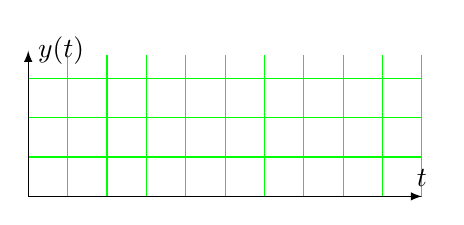
\begin{tikzpicture}

\draw[xstep=0.5,ystep=0.5,green] (0,0) grid (5,1.8);

\draw[-latex] (0,0) -- (5,0)node[above](t){$t$};
\draw[-latex] (0,0) -- (0,1.85)node[ right]{$y(t)$};
\RepTemp[color=red,samples=100,smooth,ultra thick,name path=S
]{0:5}{
0.3*x+0.15*sin(5*x)
}
\end{tikzpicture}
\sq Que peut-on dire de $\lim\limits_{y\to\infty}(y(t))$?

La réponse temporelle oscille autour d'une droite. Elle n'a pas de limite finie pour une entrée constante.






\partie*{Asservissement de position}

\subpartie*{Boucle de vitesse}


\qst Reproduire le schéma-blocs limité à cette boucle. Préciser la chaîne directe et la chaîne de retour.

%===============Cor============

{\smaller
\begin{tikzpicture}
\sbEntree{Vc}
\sbComp{C2}{Vc}				\sbRelier[$U_v(p)$]{Vc}{C2}

\sbBloc[5]{H1}{$\dfrac{K_v\cdot A\cdot G\cdot \delta}{1+\dfrac{p^2}{\beta^2}}$}{C2}
									\sbRelier{C2}{H1}
									
\sbSortie{V}{H1}					\sbRelier[$V(p)$]{H1}{V}

\sbDecaleNoeudy[5]{H1}{R1}
\sbBlocr[0]{R1}{$g\cdot(1+\tau\cdot p)$}{R1}
									\sbRelieryx{H1-V}{R1}
									\sbRelierxy{R1}{C2}

\end{tikzpicture}\par
}

avec $CD(p)=\dfrac{K_v\cdot A\cdot G\cdot \delta}{1+\dfrac{p^2}{\beta^2}}$  et $CR(p)=g\cdot(1+\tau\cdot p)$



\qst Déterminer la fonction de transfert : $H_v(p)=\dfrac{V(p)}{U_v(p)}$



On applique la formule de Black

\begin{align*}
H_v(p)&=\dfrac{V(p)}{U_v(p)}=\dfrac{CD(p)}{1+CD(p)\cdot CR(p)}\\
&=\dfrac{\dfrac{K_v\cdot A\cdot G\cdot \delta}{1+\dfrac{p^2}{\beta^2}}}{1+\dfrac{K_v\cdot A\cdot G\cdot \delta}{1+\dfrac{p^2}{\beta^2}}\cdot g\cdot(1+\tau\cdot p)}
\end{align*}


\begin{align*}
H_v(p)&=\dfrac{K_v\cdot A\cdot G\cdot \delta}{{1+\dfrac{p^2}{\beta^2}}+K_v\cdot A\cdot G\cdot \delta\cdot g\cdot(1+\tau\cdot p)}\\
H_v(p)&=\dfrac{K_v\cdot A\cdot G\cdot \delta}{{1+K_v\cdot A\cdot G\cdot \delta\cdot g+K_v\cdot A\cdot G\cdot \delta\cdot g\cdot\tau\cdot p+\dfrac{p^2}{\beta^2}}}\\
H_v(p)&=\dfrac{\dfrac{K_v\cdot A\cdot G\cdot \delta}{1+K_v\cdot A\cdot G\cdot \delta\cdot g}}{1+\dfrac{K_v\cdot A\cdot G\cdot \delta\cdot g\cdot\tau}{1+K_v\cdot A\cdot G\cdot \delta\cdot g}\cdot p+\dfrac{p^2}{(1+K_v\cdot A\cdot G\cdot \delta\cdot g)\cdot\beta^2}}
\end{align*}




Compte tenu des valeurs numériques et quelques arrondis, on obtient:

\begin{align*}
H_v(p)&=\dfrac{\num{0.094}\cdot K_v}{1+\num{0.94}\cdot K_v}\dfrac{1}{1+\dfrac{\num{0.94}\cdot K_v\cdot\tau}{1+\num{0.94}\cdot K_v}\cdot p+\dfrac{p^2}{(1+\num{0.94}\cdot K_v)\cdot\beta^2}}
\end{align*}



\qst Déterminer pour chaque réponse temporelle, $T_{5\%}$: le temps de réponse à 5\%, $D_{1\%}$: le premier dépassement relatif  et la valeur finale.


Voir la figure~\ref{fig:trainPendulaire-reptemp-c}  page~\pageref{fig:trainPendulaire-reptemp-c}.




On souhaite que cette boucle de vitesse soit la plus rapide possible et que le premier dépassement soit inférieur à 10\%.

\qst Proposer un réglage de $\tau$   et $K_v$.

La solution qui semble la meilleure parmi tous ces essais est [$\tau =\SI{0.42e-2}{\second}$, $K_v = 21$ (figure~\ref{fig:trainPendulaire-reptemp4c}).



\begin{figure}[!htb]
\centering

\subfloat[$\tau =\SI{0.42e-2}{\second}$, $K_v = 42$]{

\begin{tikzpicture}[xscale=180,yscale=7]

\draw[xstep=0.005,ystep=0.05,green] (0,0) grid (0.04,1.2);

\draw[-latex] (0,0) -- (0.042,0)node[above](t){$t$};
\draw[-latex] (0,0) -- (0,1.25)node[ right]{$v(t)$};
%\draw[dashed,blue,ultra thick] (0,1) -- (0.05,1);

\RepTemp[color=black,samples=100,smooth,ultra thick,name path=S
]{0:0.04}{
10*(0.975e-1-0.974e-1*exp(-492.*x)*cosh(40.3*x)-1.19*exp(-492.*x)*sinh(40.3*x))
}

\foreach \nn in {0,1,...,4}{
\node[below]at (0.0\nn,0){\num{0.0\nn}};
}
\foreach \nn in {0.2, 0.4, 0.6, 0.8,1,1.2}{
\node[left]at (0,\nn){\num{\nn}};
}

\def\VF{0.97}
\draw[dashed,red,thin] (0,\VF) --++ (0.04,0)node[right]{\num{\VF}};
\draw[dashed,red, name path=D95,ultra thick] (0,{\VF*0.95}) --++ (0.04,0)node[below left]{$\num{0.95}\cdot \num{\VF}$};
\draw[dashed,red, name path=D105,ultra thick] (0,{\VF*1.05}) --++ (0.04,0)node[above left]{$\num{1.05}\cdot \num{\VF}$};
%

\path [name intersections={of=D95 and S,by=E}];
%\path [name intersections={of=D105 and S}];
\draw (E) -- (E|-0,0) node[below=1em]{$T_{5\%}\approx\SI{0.01}{\second}$};

\node[fill=white, above left=1em and 2em of t,minimum width=2.5cm, minimum height=3cm,text width=5cm]{Valeur finale:  $\SI{\VF}{\metre\per\second}$  \\[2em]
$T_{5\%}\approx\SI{0.01}{\second}$ \\[2em]
$D_{1\%}$: $\varnothing$
};
\end{tikzpicture}
}
\subfloat[$\tau =\SI{0.42e-2}{\second}$, $K_v = 21$]{\label{fig:trainPendulaire-reptemp4c}

\begin{tikzpicture}[xscale=180,yscale=7]

\draw[xstep=0.05,ystep=0.05,green] (0,0) grid (0.04,1.2);

\draw[-latex] (0,0) -- (0.042,0)node[above](t){$t$};
\draw[-latex] (0,0) -- (0,1.25)node[ right]{$v(t)$};
%\draw[dashed,blue,ultra thick] (0,1) -- (0.05,1);

\RepTemp[color=black,samples=100,smooth,ultra thick,name path=S
]{0:0.04}{
10*(0.952e-1-0.954e-1*exp(-246.*x)*cos(250.*x)-0.938e-1*exp(-246.*x)*sin(250.*x))
}


\foreach \nn in {0,1,...,4}{
\node[below]at (0.0\nn,0){\num{0.0\nn}};
}
\foreach \nn in {0.2, 0.4, 0.6, 0.8,1,1.2}{
\node[left]at (0,\nn){\num{\nn}};
}

\def\VF{0.95}
\draw[dashed,red,thin] (0,\VF) --++ (0.04,0)node[right]{\num{\VF}};
\draw[dashed,red, name path=D95,ultra thick] (0,{\VF*0.95}) --++ (0.04,0)node[below left]{$\num{0.95}\cdot \num{\VF}$};
\draw[dashed,red, name path=D105,ultra thick] (0,{\VF*1.05}) --++ (0.04,0)node[above left]{$\num{1.05}\cdot \num{\VF}$};

\path [name intersections={of=D95 and S,by=E}];
%\path [name intersections={of=D105 and S}];
\draw (E) -- (E|-0,0) node[below=1em]{$T_{5\%}\approx\SI{0.008}{\second}$};

\node[fill=white, above left=1em and 2em of t,minimum width=2.5cm, minimum height=3cm,text width=5cm]{Valeur finale:   $\SI{\VF}{\metre\per\second}$  \\[2em]
$T_{5\%}\approx\SI{0.008}{\second}$ \\[2em]
$D_{1\%}= 5\%$
};
\end{tikzpicture}
}


\subfloat[$\tau =\SI{0.21e-2}{\second}$, $K_v = 21$]{

\begin{tikzpicture}[xscale=180,yscale=7]

\draw[xstep=0.005,ystep=0.05,green] (0,0) grid (0.04,1.2);

\draw[-latex] (0,0) -- (0.042,0)node[above](t){$t$};
\draw[-latex] (0,0) -- (0,1.25)node[ right]{$v(t)$};
%\draw[dashed,blue,ultra thick] (0,1) -- (0.05,1);

\RepTemp[color=black,samples=100,smooth,ultra thick,name path=S
]{0:0.04}{
10*(0.952e-1-0.952e-1*exp(-123.*x)*cos(328.*x)-0.356e-1*exp(-123.*x)*sin(328.*x))
}


\foreach \nn in {0,1,...,4}{
\node[below]at (0.0\nn,0){\num{0.0\nn}};
}
\foreach \nn in {0.2, 0.4, 0.6, 0.8,1,1.2}{
\node[left]at (0,\nn){\num{\nn}};
}

\def\VF{0.95}
\draw[dashed,red,thin] (0,\VF) --++ (0.04,0)node[right]{\num{\VF}};
\draw[dashed,red, name path=D95,ultra thick] (0,{\VF*0.95}) --++ (0.04,0)node[below left]{$\num{0.95}\cdot \num{\VF}$};
\draw[dashed,red, name path=D105,ultra thick] (0,{\VF*1.05}) --++ (0.04,0)node[above left]{$\num{1.05}\cdot \num{\VF}$};

\path [name intersections={of=D95 and S}];
%\path [name intersections={of=D105 and S}];
\draw (intersection-3) -- (intersection-3|-0,0) node[below=1em]{$T_{5\%}\approx\SI{0.0225}{\second}$};

\node[fill=white, above left=1em and 2em of t,minimum width=2.5cm, minimum height=3cm,text width=5cm]{Valeur finale: $\SI{\VF}{\metre\per\second}$  \\[2em]
$T_{5\%}\approx\SI{0.0225}{\second}$ \\[2em]
$D_{1\%}=\dfrac{\num{1.25}-\VF}{\VF}\approx 30\%$:
};
\end{tikzpicture}
}
\subfloat[$\tau =\SI{0.84e-2}{\second}$, $K_v = 42$]{

\begin{tikzpicture}[xscale=180,yscale=7]

\draw[xstep=0.005,ystep=0.05,green] (0,0) grid (0.04,1.2);

\draw[-latex] (0,0) -- (0.042,0)node[above](t){$t$};
\draw[-latex] (0,0) -- (0,1.25)node[ right]{$v(t)$};
%\draw[dashed,blue,ultra thick] (0,1) -- (0.05,1);

\RepTemp[color=black,samples=100,smooth,ultra thick,name path=S
]{0:0.04}{
10*(0.975e-1-0.975e-1*exp(-983.*x)*cosh(852.*x)-.112*exp(-983.*x)*sinh(852.*x))
}


\foreach \nn in {0,1,...,4}{
\node[below]at (0.0\nn,0){\num{0.0\nn}};
}
\foreach \nn in {0.2, 0.4, 0.6, 0.8,1,1.2}{
\node[left]at (0,\nn){\num{\nn}};
}

\def\VF{0.97}
\draw[dashed,red,thin] (0,\VF) --++ (0.04,0)node[right]{\num{\VF}};
\draw[dashed,red, name path=D95,ultra thick] (0,{\VF*0.95}) --++ (0.04,0)node[below left]{$\num{0.95}\cdot \num{\VF}$};
\draw[dashed,red, name path=D105,ultra thick] (0,{\VF*1.05}) --++ (0.04,0)node[above left]{$\num{1.05}\cdot \num{\VF}$};

\path [name intersections={of=D95 and S,by=E}];
%\path [name intersections={of=D105 and S}];
\draw (E) -- (E|-0,0) node[below=1em]{$T_{5\%}\approx\SI{0.023}{\second}$};

\node[fill=white, above left=1em and 2em of t,minimum width=2.5cm, minimum height=3cm,text width=5cm]{Valeur finale:  $\SI{\VF}{\metre\per\second}$  \\[2em]
$T_{5\%}\approx\SI{0.023}{\second}$ \\[2em]
$D_{1\%}$: $\varnothing$
};
\end{tikzpicture}
}
\caption{Réponse temporelle de la boucle de vitesse pour une consigne de $u_v(t)=\SI{10}{\volt}$  pour différentes valeurs de $K_v$  et $\tau$.}
\label{fig:trainPendulaire-reptemp-c}
\end{figure}



\qst Quelle doit être la valeur du gain d'adaptation de la consigne $A_d$  pour que l'asservissement fonctionne correctement?

Il faut $A_d=h$


\qst Modifier le schéma-blocs pour le mettre sous la forme suivante:

{
\begin{tikzpicture}
\sbEntree{Yc}
\sbComp[3]{C1}{Yc}				\sbRelier[$Y_c(p)$]{Yc}{C1}
\sbBloc{BO}{$ \dfrac{23250 \cdot K_p \cdot h }{p\cdot(p+488)^2}$}{C1}\sbRelier{C1}{BO}
\sbSortie{Y}{BO}					\sbRelier[$Y(p)$]{BO}{Y}

\sbRenvoi[3]{BO-Y}{C1}{}

\end{tikzpicture}\par
}


\qst Déterminer $BO(p)$


\begin{align*}
BO(p)&= \dfrac{23250 \cdot K_p \cdot h }{p\cdot(p+488)^2}
\end{align*}

\qst Déterminer la fonction de transfert en boucle fermée $H_p(p)=\dfrac{Y(p)}{Y_c(p)}$

\begin{align*}
H_p(p)&=\dfrac{BO(p)}{1+BO(p)}= \dfrac{\dfrac{23250 \cdot K_p \cdot h }{p\cdot(p+488)^2}}{1+\dfrac{23250 \cdot K_p \cdot h }{p\cdot(p+488)^2}}\\
H_p(p)&= \dfrac{23250 \cdot K_p \cdot h }{p\cdot(p+488)^2+23250 \cdot K_p \cdot h }\\
H_p(p)&= \dfrac{23250 \cdot K_p \cdot h }{p^3+976\cdot p^2 +488^2\cdot p+23250 \cdot K_p \cdot h }\\
H_p(p)&= \dfrac{1}{\dfrac{p^3}{23250 \cdot K_p \cdot h }+\dfrac{976\cdot p^2}{23250 \cdot K_p \cdot h } +\dfrac{488^2\cdot p}{23250 \cdot K_p \cdot h }+1}\\
\end{align*}

 $K_p=\num{0.9}$.


La fonction de transfert devient (avec quelques arrondis!):

\begin{align*}
H_p(p)&=\dfrac{1}{\left(\dfrac{p}{532}+1\right)\cdot \left(\dfrac{p}{439}+1\right)\cdot\left (\dfrac{p}{4.5}+1\right)}
\end{align*}

On sollicite avec un échelon unitaire $y(t)=Y_0\cdot \heav$  avec $Y_0=\SI{0.1}{\metre}$.

\qst Montrer que $Y(p)$  s'écrit 

\begin{align*}
Y(p)&= \dfrac{A}{\dfrac{p}{532}+1}+\dfrac{B}{\dfrac{p}{439}+1}+ \dfrac{C}{\dfrac{p}{4.5}+1} +\dfrac{D}{p}\\
Y(p)&=\dfrac{Y_0}{\left(\dfrac{p}{532}+1\right)\cdot \left(\dfrac{p}{439}+1\right)\cdot\left (\dfrac{p}{4.5}+1\right)\cdot p}
\end{align*}

On multiplie de chaque coté de l'égalité par $\left(\dfrac{p}{532}+1\right)$  puis on prend $p=-532$.

on obtient
\begin{align*}
 {A}&
=\dfrac{Y_0}{ \left(\dfrac{-532}{439}+1\right)\cdot\left (\dfrac{-532}{4.5}+1\right)\cdot (-532)}\\
A&=-\dfrac{1317}{17399060}\cdot Y_0\approx \num{-0.757e-4}\cdot Y_0
\end{align*}
de même pour $B$  et $C$.
\begin{align*}
B&=\dfrac{1596}{11826221}\cdot Y_0\approx \num{0.135e-3} \cdot Y_0\\
C&=\num{-.22643}\cdot Y_0
\end{align*}
et 
\begin{align*}
D&=1
\end{align*}

\qst Déterminer $y(t)$.

À partir du tableau des transformées

\begin{align*}
y(t)=Y_0\cdot\Big(1-\dfrac{1317}{32705}\cdot e^{-532\cdot t}&+\dfrac{1596}{26939}\cdot e^{-439\cdot t}\\
&-\dfrac{934192}{916795}\cdot e^{-\num{4.5}\cdot t}\Big)\cdot \heav
\end{align*}
\begin{align*}
y(t)\approx Y_0\cdot\Big(1-0.040 \cdot e^{-532\cdot t}&+0.059\cdot e^{-439\cdot t}\\
&-1.02\cdot e^{-\num{4.5}\cdot t}\Big)\cdot \heav
\end{align*}




\qst À partir de la réponse temporelle ci-dessous, préciser, l'erreur indicielle, le temps de réponse.

\begin{tikzpicture}[xscale=3.5,yscale=50]

\draw[xstep=0.2,ystep=0.005,green] (0,0) grid (2,0.12);

\draw[-latex] (0,0) -- (2,0)node[above](t){$t$};
\draw[-latex] (0,0) -- (0,0.125)node[ right]{$y(t)$};
%\draw[dashed,blue,ultra thick] (0,1) -- (0.05,1);

\RepTemp[color=red,samples=100,smooth,ultra thick,name path=S
]{0:2}{
0.1*(1 -0.400e-1*exp(-532.*x)+0.588e-1*exp(-439.*x)-1.02*exp(-4.48*x))
}

\RepTemp[color=blue,dashed,samples=100,smooth,ultra thick,name path=S
]{0:2}{
0.1*(1 -1.02*exp(-4.48*x))
}

\foreach \nn in {0,1,2}{
\node[below]at (\nn,0){\num{\nn}};
}
\foreach \nn in {0.02, 0.04, 0.06, 0.08,0.1,0.12}{
\node[left]at (0,\nn){\num{\nn}};
}

\def\VF{0.1}
\draw[dashed,red,thin] (0,\VF) --++ (2,0)node[right]{\num{\VF}};
\draw[dashed,red, name path=D95,ultra thick] (0,{\VF*0.95}) --++ (2,0)node[below left]{$\num{0.95}\cdot \num{\VF}$};
\draw[dashed,red, name path=D105,ultra thick] (0,{\VF*1.05}) --++ (2,0)node[above left]{$\num{1.05}\cdot \num{\VF}$};

\path [name intersections={of=D95 and S,by=E}];
%\path [name intersections={of=D105 and S}];
\draw (E) -- (E|-0,0) node[below=1em]{$T_{5\%}\approx\SI{0.7}{\second}$};

\node[fill=white, above left=1em and 2em of t,minimum width=2.5cm, minimum height=3cm,text width=4cm]{Erreur indicielle: $\varepsilon_i=0$  \\[2em]
$T_{5\%}\approx\SI{0.7}{\second}$: \\[2em]
$D_{1\%}$: $\varnothing$
};
\end{tikzpicture}



\qst Montrer que la fonction de transfert en boucle fermée obtenue peut être simplifiée par \begin{align*}
H_{ps}(p) &=\dfrac{1}{\dfrac{p}{4.5}+1}
\end{align*}

Les deux exponentielles  $\cdot e^{-532\cdot t}$  et $e^{-439\cdot t}$  sont très rapidement nulles.

La réponse temporelle est alors peu différente de 
\begin{align*}
y(t)\approx Y_0\cdot\Big(1-1.02\cdot e^{-\num{4.5}\cdot t}\Big)\cdot \heav
\end{align*}

La courbe correspondante est tracée sur le graphe ci-dessus.

La fonction de transfert simplifiée s'écrit donc:

\begin{align*}
H_{ps}(p) &=\dfrac{1}{\dfrac{p}{4.5}+1}
\end{align*}


\end{multicols}



\end{Cor}



\end{Exo}
